% \begin{table}[t]
% \centering
% \caption{Forward and backward speed of DiffVG \cite{Li:2020:DVG} and Bézier splatting (tested on a 2,040$\times$1,344 image, using 2,048 curves).}
% \vspace{-1em}
% \resizebox{0.95\linewidth}{!}{%
% \begin{tabular}{ll|ccc}
% \hline
%  & & DiffVG & Bézier splatting & Speedup \\
% \hline
% \multirow{2}{*}{Open} & Forward & 141.3ms  & \textbf{7.2ms} & 19.6$\times$ \\  
% & Backward & 701.3.ms & \textbf{4.7ms} & 149.2$\times$ \\  
% \hline
% \multirow{2}{*}{Closed} & Forward & 85.2ms  & \textbf{14.2ms} & 6.0$\times$ \\  
% & Backward & 448.3ms  & \textbf{15.7ms} & 28.5$\times$ \\  
% \hline
% \end{tabular}
% }
% \label{tab:speed_comparison}
% \vspace{-.5em}
% \end{table}

\begin{table}[t]
\centering
\caption{Computational speed for rendering a 2,040$\times$1,344 image with 2,048 curves.}
\vspace{-.7em}
\resizebox{0.83\linewidth}{!}{%
\begin{tabular}{l|ccc|ccc}
\hline
& \multicolumn{3}{c|}{\textbf{Open curve}} & \multicolumn{3}{c}{\textbf{Closed curve}} \\
& DiffVG \cite{Li:2020:DVG} & Bézier Splatting & Speedup & DiffVG \cite{Li:2020:DVG} & Bézier Splatting & Speedup \\
\hline
Forward pass & 141.3ms & \textbf{4.5ms} & \textit{31.4}$\times$ & 85.2ms & \textbf{14.1ms} & \textit{6.0}$\times$ \\
Backward pass & 701.3ms & \textbf{4.7ms} & \textit{149.2}$\times$ & 448.3ms & \textbf{24.58ms} & \textit{18.2}$\times$ \\
\hline
\end{tabular}
}
\label{tab:speed_comparison}
% \vspace{-.5em}
\end{table}



\begin{figure}[!t]
\centering
% \vspace{-2em}
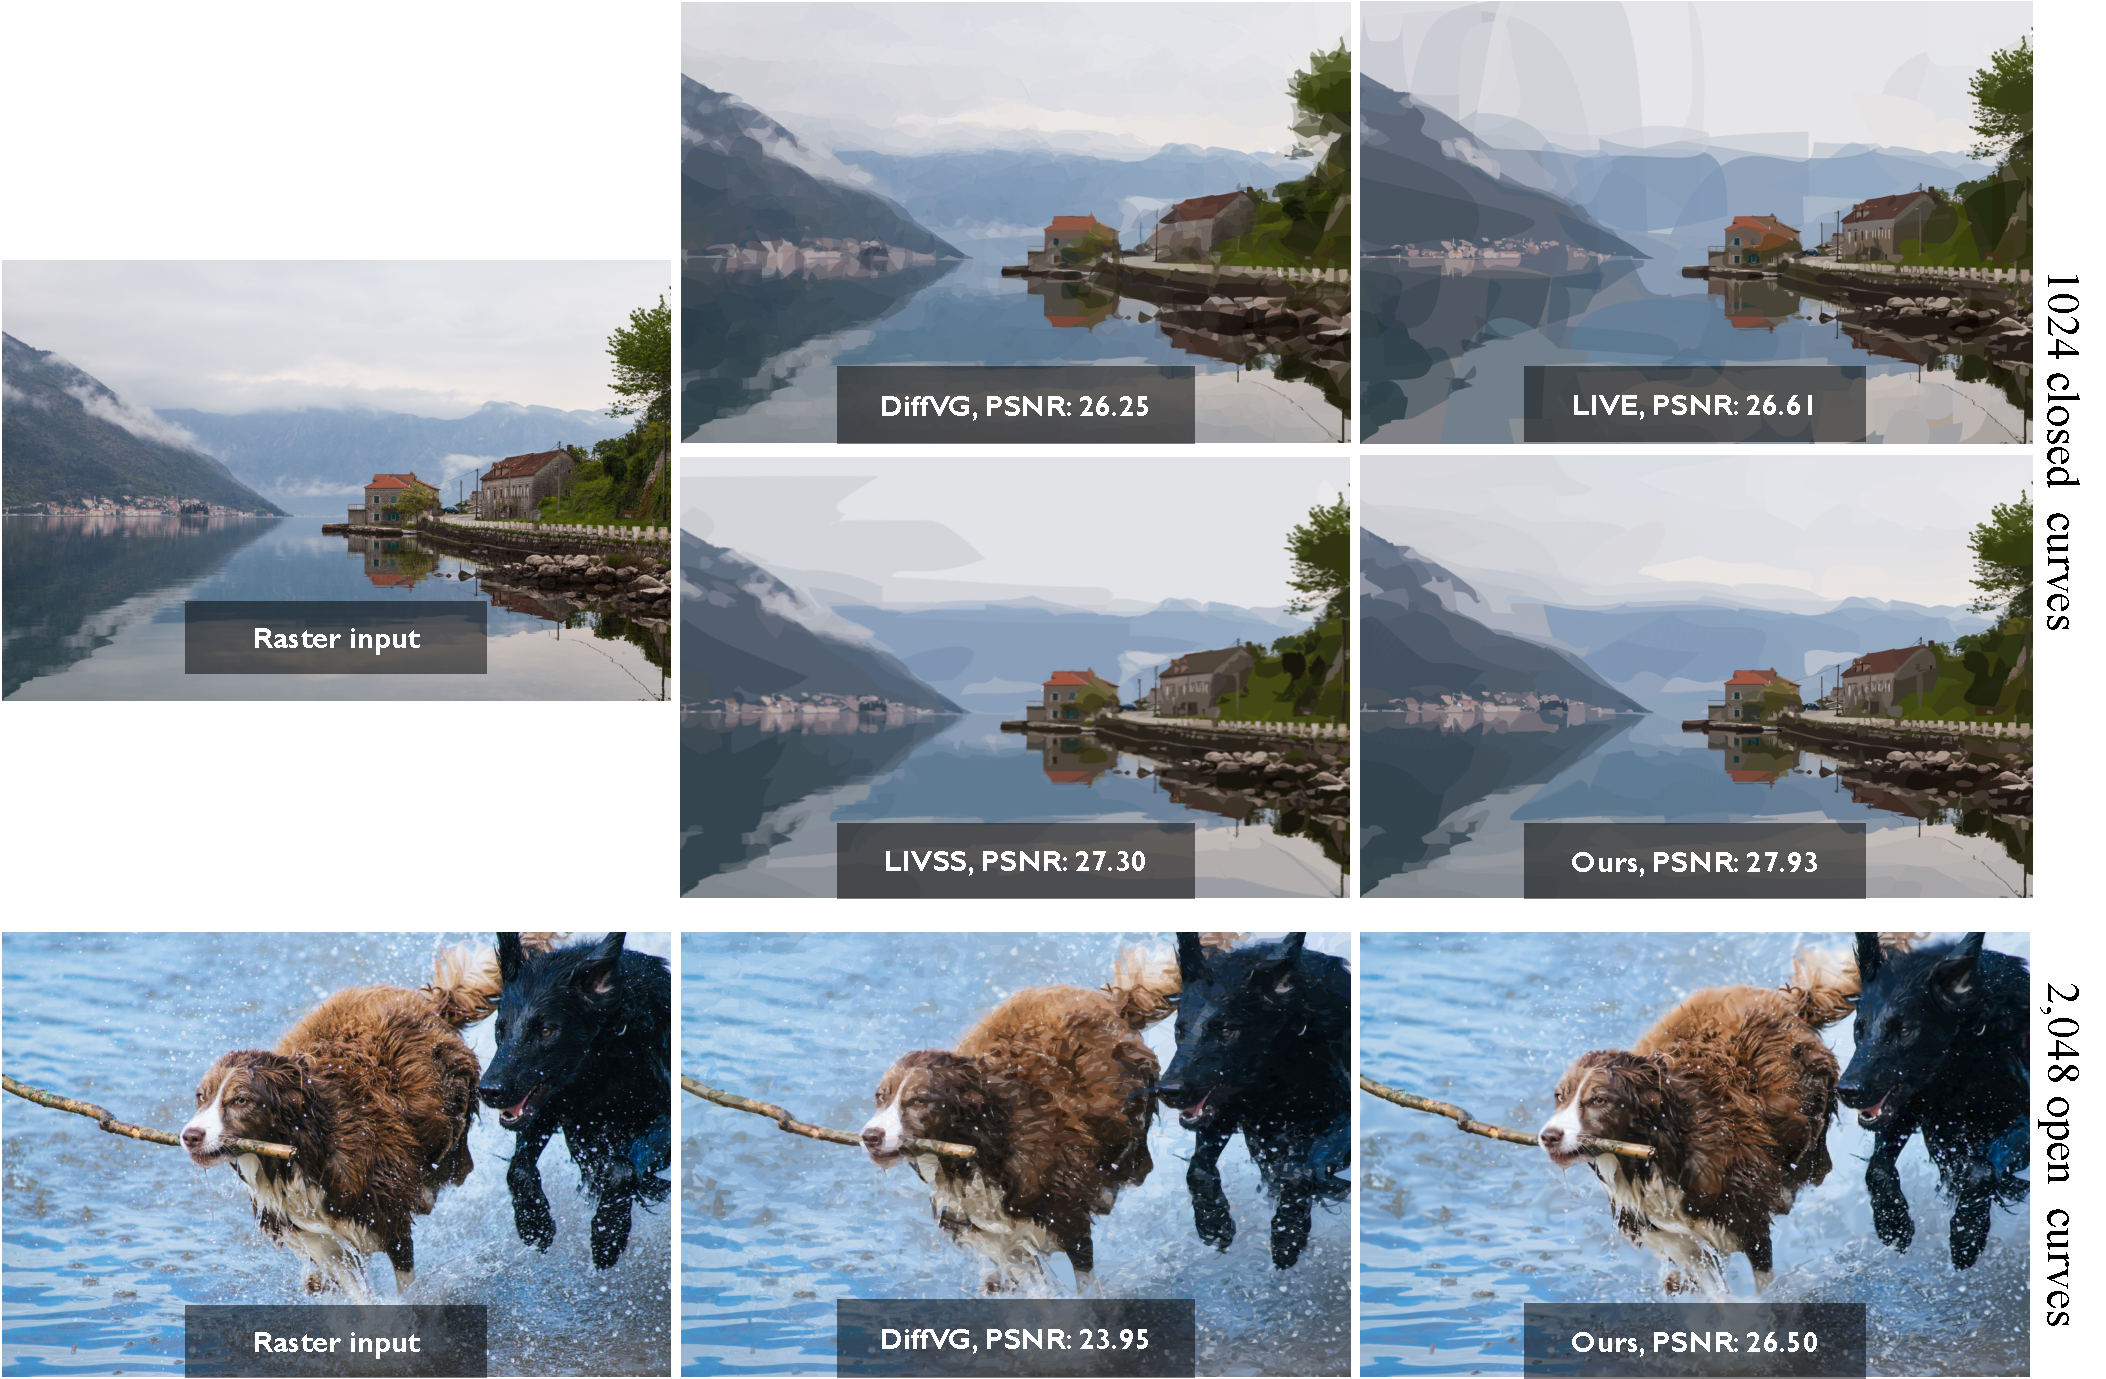
\includegraphics[width=0.98\linewidth]{figures/comparison_v2.pdf}
\vspace{-.5em}
\caption{A qualitative comparison of our method and the state-of-the-art differentiable VG rasterization methods, including DiffVG \cite{Li:2020:DVG},  LIVE \cite{xu2022live}, and LIVSS \cite{livss}.
% , with different number ($N$) of open and closed curves. 
% The raster input is taken from the DIV2K dataset \cite{Timofte_2017_CVPR_Workshops}.
}
\label{fig:comparison}
\vspace{-.5em}
\end{figure}

\vspace{-.5em}
\section{Experiments}
\vspace{-.5em}

\subsection{Experimental Setups}
\noindent\textbf{Implementation details.} We implement Bézier Splatting in PyTorch \cite{paszke2019pytorch} and optimize it by using the Adam optimizer \cite{2015-kingma} with a StepLR learning rate scheduler. The learning rate is initialized at 0.01 for color, 2e-4 for Bézier curve control points, and 0.1 for opacity. For the pruning and densification strategy, the opacity threshold is set to 0.02, and the overlap threshold based on Axis-Aligned Bounding Boxes (AABB) is set to 0.9. Following the approach in LIVE \cite{xu2022live}, new curves are initialized in a circular pattern, and the number of added curves matches the number of removed ones to maintain a constant total curve count. Open curves are optimized for 15,000 iterations, and closed curves are optimized for 10,000 iterations. Pruning and densification are applied every 400 steps until the last but 1,000 steps, after which they are halted to stabilize the representation. 

\noindent\textbf{Datasets.} We comprehensively evaluate our method across different image domains. We use the publicly available DIV2K \cite{Timofte_2017_CVPR_Workshops} dataset for evaluating natural images. Due to the high computational cost of baseline method LIVE \cite{xu2022live}, we uniformly subsample the DIV2K dataset by selecting one out of every four images, resulting in a final evaluation set of 200 images from the original 800-image dataset.
Additionally, we test our method on non-photorealistic images, including the artwork images from Clipart1K dataset \cite{inoue2018cross} and cartoon images from Danbooregions dataset \cite{DanbooRegion2020}, to demonstrate its effectiveness for diverse types of images, as shown in Fig. \ref{fig:showcase}. 

\begin{table*}[!t]
\centering
\caption{
    \label{tab:comparisons_div2k} Quantitative evaluation and optimization efficiency of differentiable VG methods on the DIV2K dataset \cite{Timofte_2017_CVPR_Workshops}.
}
\setlength{\tabcolsep}{3pt}
\resizebox{0.99\textwidth}{!}{
\begin{tabular}{l|l|cccc|cccc|cccc}
\hline
& \multirow{2}{*}{\textbf{Method}} 
& \multicolumn{4}{c|}{\textbf{256 curves}} 
& \multicolumn{4}{c|}{\textbf{512 curves}} 
& \multicolumn{4}{c}{\textbf{1024 curves}} \\
& & $SSIM^\uparrow$ & $PSNR^\uparrow$ & $LPIPS^\downarrow$ & \cellcolor{timegray}$\text{Opt.}^\downarrow$
  & $SSIM^\uparrow$ & $PSNR^\uparrow$ & $LPIPS^\downarrow$ & \cellcolor{timegray}$\text{Opt.}^\downarrow$
  & $SSIM^\uparrow$ & $PSNR^\uparrow$ & $LPIPS^\downarrow$ & \cellcolor{timegray}$\text{Opt.}^\downarrow$ \\
\hline

\multirow{2}{*}{Open} 
& DiffVG~\cite{Li:2020:DVG} 
  & \cellcolor{baselinegray}0.552 & \cellcolor{baselinegray}19.83 & \cellcolor{baselinegray}0.563 & \cellcolor{timegray}18.9min 
  & \cellcolor{baselinegray}0.587 & \cellcolor{baselinegray}21.47 & \cellcolor{baselinegray}0.537 & \cellcolor{timegray}22.0min 
  & \cellcolor{baselinegray}0.616 & \cellcolor{baselinegray}22.62 & \cellcolor{baselinegray}0.517 & \cellcolor{timegray}30.6min \\
& Ours 
  & \cellcolor{oursblue}\textbf{0.600} & \cellcolor{oursblue}\textbf{22.17} & \cellcolor{oursblue}\textbf{0.540} & \cellcolor{timegray}\textbf{3.4min}
  & \cellcolor{oursblue}\textbf{0.646} & \cellcolor{oursblue}\textbf{23.79} & \cellcolor{oursblue}\textbf{0.498} & \cellcolor{timegray}\textbf{3.3min}
  & \cellcolor{oursblue}\textbf{0.699} & \cellcolor{oursblue}\textbf{25.45} & \cellcolor{oursblue}\textbf{0.448} & \cellcolor{timegray}\textbf{3.2min} \\
\hline

\multirow{4}{*}{Closed} 
& DiffVG~\cite{Li:2020:DVG}
  & \cellcolor{baselinegray}0.578 & \cellcolor{baselinegray}20.69 & \cellcolor{baselinegray}0.548 & \cellcolor{timegray}16.4min
  & \cellcolor{baselinegray}0.601 & \cellcolor{baselinegray}21.82 & \cellcolor{baselinegray}0.531 & \cellcolor{timegray}18.5min
  & \cellcolor{baselinegray}0.631 & \cellcolor{baselinegray}22.95 & \cellcolor{baselinegray}0.509 & \cellcolor{timegray}25.1min \\
& LIVE~\cite{xu2022live} 
  & \cellcolor{baselinegray}0.576 & \cellcolor{baselinegray}20.09 & \cellcolor{baselinegray}0.543 & \cellcolor{timegray}2.6h
  & \cellcolor{baselinegray}0.611 & \cellcolor{baselinegray}21.70 & \cellcolor{baselinegray}\textbf{0.521} & \cellcolor{timegray}4.2h
  & \cellcolor{baselinegray}0.648 & \cellcolor{baselinegray}23.11 & \cellcolor{baselinegray}0.495 & \cellcolor{timegray}5.1h \\
& LIVSS~\cite{livss} 
  & \cellcolor{baselinegray}\textbf{0.586} & \cellcolor{baselinegray}17.71 & \cellcolor{baselinegray}\textbf{0.542} & \cellcolor{timegray}39.2min
  & \cellcolor{baselinegray}\textbf{0.630} & \cellcolor{baselinegray}18.71 & \cellcolor{baselinegray}0.530 & \cellcolor{timegray}54.3min
  & \cellcolor{baselinegray}\textbf{0.678} & \cellcolor{baselinegray}19.83 & \cellcolor{baselinegray}0.517 & \cellcolor{timegray}1.4h \\
& Ours 
  & \cellcolor{oursblue}0.580 & \cellcolor{oursblue}\textbf{20.74} & \cellcolor{oursblue}0.546 & \cellcolor{timegray}\textbf{7.8min}
  & \cellcolor{oursblue}0.607 & \cellcolor{oursblue}\textbf{22.11} & \cellcolor{oursblue}0.528 & \cellcolor{timegray}\textbf{8.3min}
  & \cellcolor{oursblue}0.639 & \cellcolor{oursblue}\textbf{23.45} & \cellcolor{oursblue}\textbf{0.507} & \cellcolor{timegray}\textbf{8.6min} \\
\hline
\end{tabular}
}
\end{table*}




% \begin{table*}[!h]
%     \centering
%     \caption{
%         \label{tab:comparisons} Quantitative evaluation of DIV2K\_HR
%     }
%     \vspace{-.5em}
%     \resizebox{0.85\textwidth}{!}{
%         \begin{tabular}{l|l|cccc|cccc}
%         \toprule
%             & \multirow{2}{*} {\textbf{Method} / \textbf{Curve \#} } & \multicolumn{4}{c|}{\textbf{256}} & \multicolumn{4}{c}{\textbf{512}} \\
                        
%             &  & $SSIM^\uparrow$   & $PSNR^\uparrow$    & $LPIPS^\downarrow$  & Train & $SSIM^\uparrow$   & $PSNR^\uparrow$    & $LPIPS^\downarrow$  & Train \\
%             \hline
            
%             \multirow{2}{*}{Open} 
%             & DiffVG & 0.552 & 19.83 & 0.563 & 18m56s & 0.587 & 21.47 & 0.537 & 22m01s \\
%             & Bézier splatting (ours) & \textbf{0.600} & \textbf{22.17} & \textbf{0.540} & \textbf{3m37s} & \textbf{0.646} & \textbf{23.79} & \textbf{0.498} & \textbf{3m21s} \\
            
%             \hline
%             \multirow{3}{*}{Closed} 
%             & DiffVG & 0.578 & 20.69 & 0.548 & 16m27s & 0.601 & 21.82 & 0.531 & 18m35s \\
%             & LIVE  & 0.576 & 20.09 & \textbf{0.543} & 2h41m & \textbf{0.611} & 21.70 & \textbf{0.521} & 4h12m \\
%             & Bézier splatting (ours) & \textbf{0.581} & \textbf{20.74} & 0.547 & \textbf{2m22s} & \textbf{0.611} & \textbf{22.14} & 0.522 & \textbf{2m45s} \\

%             \hline
%             & \multirow{2}{*} {\textbf{Method} / \textbf{Curve \#} } & \multicolumn{4}{c|}{\textbf{1024}} & \multicolumn{4}{c}{\textbf{2048}} \\
                        
%             &  & $SSIM^\uparrow$   & $PSNR^\uparrow$    & $LPIPS^\downarrow$  & Train & $SSIM^\uparrow$   & $PSNR^\uparrow$    & $LPIPS^\downarrow$  & Train \\
%             \hline
            
%             \multirow{2}{*}{Open} 
%             & DiffVG & 0.616 & 22.62 & 0.517 & 30m38s & 0.654 & 23.89 & 0.492 & 46m36s \\
%             & Bézier splatting (ours) & \textbf{0.699} & \textbf{25.45} & \textbf{0.448} & \textbf{3m17s} & \textbf{0.756} & \textbf{27.22} & \textbf{0.389} & \textbf{3m24s} \\
            
%             \hline
%             \multirow{3}{*}{Closed} 
%             & DiffVG & 0.631 & 22.95 & 0.509 & 25m08s & 0.668 & 24.21 & 0.482 & 34m16s \\
%             & LIVE  & \textbf{0.648} & 23.11 & 0.495 & 5h6m& - & - & - & - \\
%             & Bézier splatting (ours) & \textbf{0.648} & \textbf{23.55} & \textbf{0.491} & \textbf{3m25s} & \textbf{0.690} & \textbf{24.93} & \textbf{0.454} & \textbf{4m46s} \\

%             \hline
%         \end{tabular}
%     }
% \end{table*}


\begin{figure*}[t]
\vspace{-.5em}
\centering
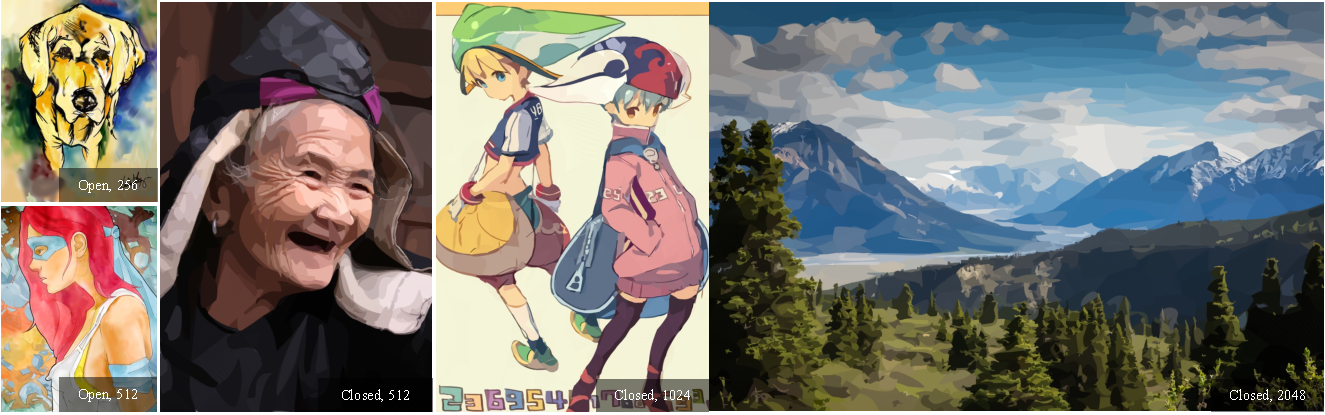
\includegraphics[width=1\linewidth]{figures/gallery.pdf}
\vspace{-1.5em}
\caption{
Our Bézier Splatting achieves high-quality image vectorization results for various types of images including artworks, cartoons, and natural images. Curve type and count are indicated at the bottom right of each sample.
% \caption{We showcase the image vectorization results by our Bézier Splatting, with open or closed curves and different curve counts indicated at the bottom right of each example. The raster inputs, shown at the top left of each example, are taken from the DIV2K \cite{Timofte_2017_CVPR_Workshops}, KIOAK \cite{kodak1999}, Clipart \cite{inoue2018cross}, and Danbooregions \cite{DanbooRegion2020} datasets. Zoom in for a better view of details.
}
\label{fig:showcase}
% \vspace{-1em}
\end{figure*}

\vspace{-.5em}
\subsection{Method Comparison}
\vspace{-.5em}

Table \ref{tab:speed_comparison} reports the forward and backward runtime for processing 2,048 curves on an image with a resolution of 2,040$\times$1,344. Compared to DiffVG \cite{Li:2020:DVG}, our method significantly accelerates VG rasterization by 31.4$\times$ faster per forward step and 149.2$\times$ faster per backward step for open curves. For closed curves, our color filling strategy requires sampling 20 additional Bézier curves per closed curve, while our method remains highly efficient, achieving 6$\times$ faster forward and 18.2$\times$ faster backward computation.





Table \ref{tab:comparisons_div2k} quantitatively evaluates the quality of differentiable VG representations by three commonly used metrics, MS-SSIM \cite{583d8b59c51a4f3e9bd0b90731111848}, PSNR, and LPIPS \cite{zhang2018perceptual}. Our method demonstrates higher optimization efficiency and rendering fidelity for both open and closed curves with different curve numbers. 


Fig. \ref{fig:comparison} visually compares DiffVG \cite{Li:2020:DVG}, LIVE \cite{Du:2023:IVE}, \cite{livss}, and our Bézier Splatting under 512 closed curves and 2048 open curves. 
% As the number of paths increases, it shows progressive enhancement in the visual details. 
Compared to DiffVG \cite{Li:2020:DVG}, our method captures significantly more fine-grained textures. Compared to LIVE \cite{xu2022live}, our method effectively enhances rendering quality, resulting in higher-fidelity results. This improvement stems from our method's ability to globally optimize all curves, rather than LIVE's layer-by-layer path-adding strategy. Compared to LIVSS \cite{livss}, our method demonstrates superior ability in preserving fine structural details, especially in text regions. Due to its heavy reliance on layer-wise semantic simplification, LIVSS struggles to optimize regions where semantic information is ambiguous or difficult to extract. Moreover, by optimizing the entire VG simultaneously, our approach ensures a cohesive and natural appearance, avoiding the accumulation of errors and inconsistencies introduced by layer-wise updates.




As shown in Fig. \ref{fig:showcase}, Bézier Splatting consistently renders high-quality VGs across various image domains from photorealistic natural images, watercolor paintings, to cartoon images. Unlike learning-based image vectorization methods \cite{lopes2019learned, reddy2021im2vec, Cao_2023_CVPR}, which can not easily generalize to out-of-domain data, our method can flexibly handle different types of images. 

\begin{figure*}[!t]
\centering
% \vspace{-2em}
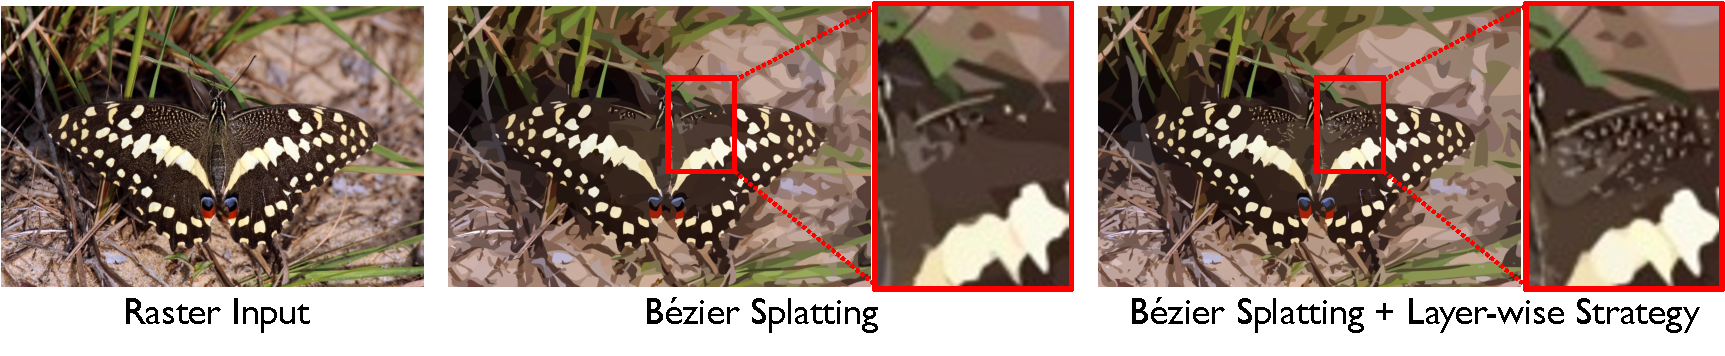
\includegraphics[width=0.92\linewidth]{figures/layerwise.pdf}
\vspace{-1em}
\caption{As a differentiable VGs renderer, Bézier Splatting can integrate with topology-aware strategies such as layer-wise vectorization \cite{xu2022live} to further improve compositionality and detail.}
\label{fig:layer}
% \vspace{-.5em}
\end{figure*}


\begin{figure*}[!t]
\centering
% \vspace{-2em}
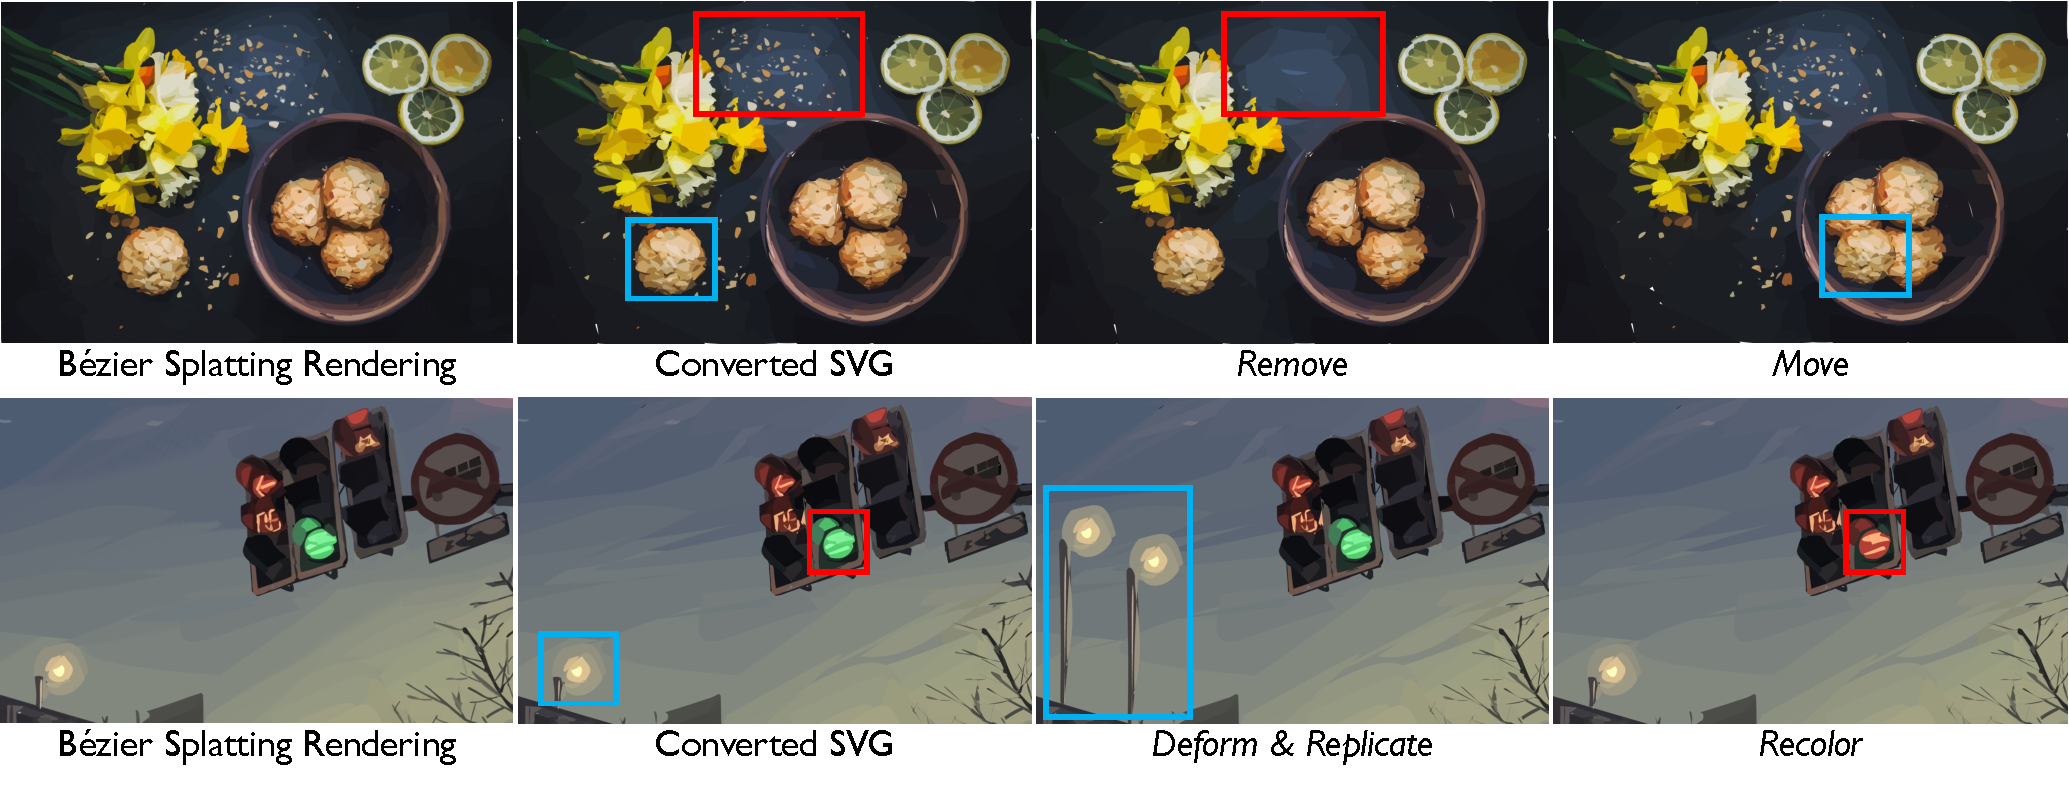
\includegraphics[width=1\linewidth]{figures/editing.pdf}
\vspace{-2em}
\caption{Our Bézier Splatting representation is compatible with the standard SVG XML format and supports flexible vector editing operations.}
\label{fig:editing}
\vspace{-.5em}
\end{figure*}


\vspace{-.5em}
\subsection{Layer-wise Image Vectorization}
Existing works such as LIVE \cite{xu2022live}, SGLIVE \cite{zhou2024segmentation} and LIVSS \cite{livss} have demonstrated that layer-wise vectorization strategies can significantly improve the topology and compositionality of DiffVG-generated vector graphics \cite{Li:2020:DVG}.
Since the proposed Bézier Splatting is a fast and differentiable VGs renderer alternative to DiffVG, is naturally compatible with these topology-aware strategies and can leverage them to further enhance the structural quality of the optimized vector outputs.
As shown in Fig. \ref{fig:layer}, we incorporate the layer-wise vectorization approach from LIVE \cite{xu2022live} into the Bézier Splatting optimization process
This integration yields improved compositional integrity and finer details for regions with complex patterns such as the butterfly's wings.

\vspace{-.5em}
\subsection{Editability and Compatibility with SVG XML Format}
Our Bézier Splatting representation is fully compatible with the standard SVG XML format, ensuring the same editability as standard SVGs and seamless integration with existing SVG tools.
As shown in Fig. \ref{fig:editing}, a high-fidelity SVG can be obtained via a simple conversion algorithm (see Appendix for details).
Once converted to SVG, the vectorized output is fully editable at the primitive level, allowing users to freely deform, remove, move, replicate, and recolor individual elements.








% \subsection{Ablation study}
% Please refer to Appendix. \ref{sec:ablation} for the ablation study.

